\subsection{Atributos seleccionados por Pearson}
La Figura \ref{Fig: PearsonAtr} muestra la nube de puntos resultante al graficar los atributos seleccionados mediante el algoritmo de Pearson. En esta representación gráfica se puede observar que los datos no presentan una segmentación notoria, y que, dado la naturaleza de los atributos \emph{hypertension} y \emph{heart\_disease} se genera un conjunto de 4 pilares, los cuales corresponden a la combinación de los 2 atributos categóricos.

\begin{figure}[htbp]
	\centering
	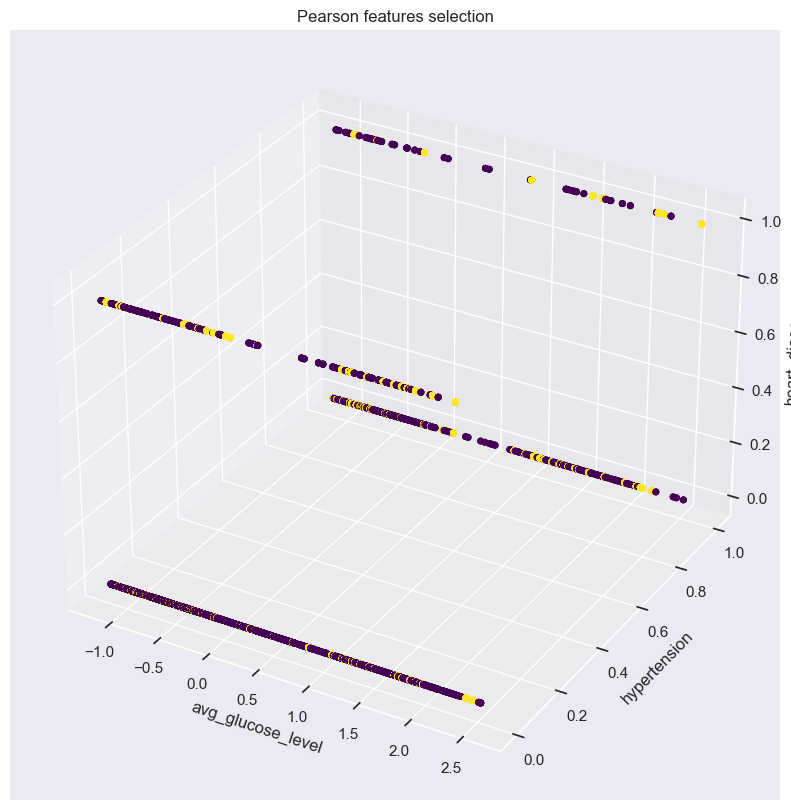
\includegraphics[width=0.8\textwidth]{pearson_features_selection}
	\caption{Atributos seleccionados por el algoritmo de Pearson.}
	\label{Fig: PearsonAtr}
\end{figure}

\subsection{Atributos seleccionados por PCA}
La Figura \ref{Fig: PCAAtr} muestra la nube de puntos resultante de los 3 componentes principales obtenidos mediante PCA. Se puede observar un aislamiento de diversas regiones, sin embargo, también se logran observar puntos donde se mezclan las clases.

\begin{figure}[htbp]
	\centering
	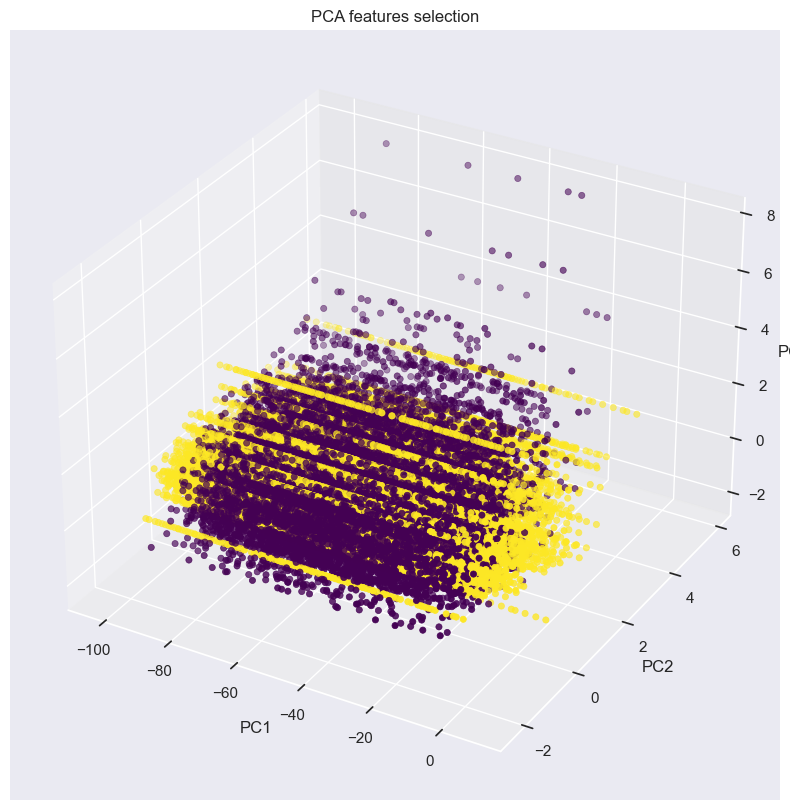
\includegraphics[width=0.8\textwidth]{pca_features_selection}
	\caption{Atributos seleccionados por el algoritmo de PCA.}
	\label{Fig: PCAAtr}
\end{figure}

\FloatBarrier
\newpage
\subsection{Atributos seleccionados por selección experimental}
Relacionado al método experimental desarrollado para esta práctica, se determinó que los atributos \emph{age}, \emph{avg\_glucose\_level} y \emph{bmi} serían los mejores. La Figura \ref{Fig: ExpAtr} muestra la nube de puntos resultante de dichos atributos, donde se puede observar que la naturaleza continua de los atributos genera una nube de puntos con áreas donde prevalece una determinada clase.

\begin{figure}[htbp]
	\centering
	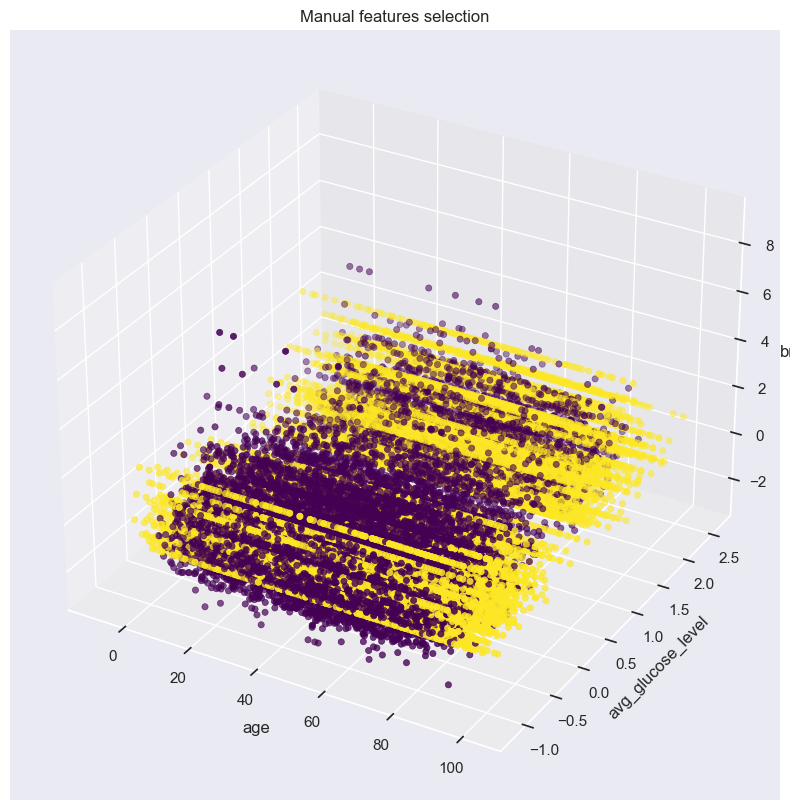
\includegraphics[width=0.8\textwidth]{manual_features_selection}
	\caption{Atributos seleccionados por selección experimental.}
	\label{Fig: ExpAtr}
\end{figure}

\FloatBarrier
\newpage
\subsection{KNN con atributos de Pearson}
Los resultados obtenidos tras la evaluación del algoritmo utilizando los atributos seleccionados mediante el algoritmo de Pearson pueden observarse en la Figura \ref{Fig: PearsonCM} y en la Tabla \ref{Tab: ResPearson}

\begin{figure}[htbp]
	\centering
	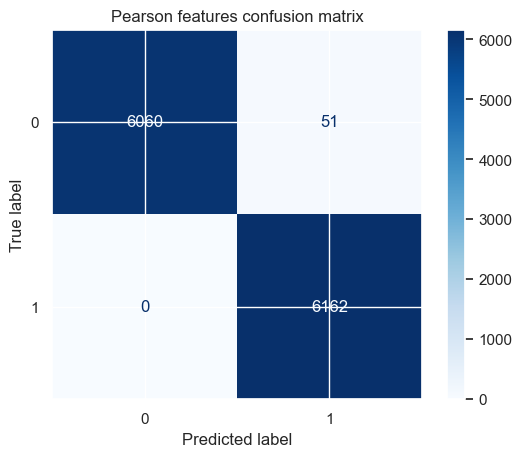
\includegraphics[width=0.6\textwidth]{pearson_features_confusion_matrix}
	\caption{Matriz de confusión resultante tras la evaluación de KNN con atributos seleccionados por Pearson.}
	\label{Fig: PearsonCM}
\end{figure}

\begin{table}[htbp]
	\centering
	\caption{Métricas de desempeño del algoritmo KNN con atributos seleccionados por Pearson.}
	\begin{tabular}{cccc}
		\hline\hline
		Exactitud    & Sensibilidad   & Precisión & Puntaje F1    \\ 
		\hline\hline
		99.58\% & 100\% & 99.18\% & 99.59\% \\
		\hline\hline
	\end{tabular}
	\label{Tab: ResPearson}
\end{table}

\newpage
\subsection{KNN con atributos de PCA}
Los resultados obtenidos tras la evaluación del algoritmo utilizando los atributos seleccionados mediante el algoritmo de PCA pueden observarse en la Figura \ref{Fig: PCACM} y en la Tabla \ref{Tab: ResPCA}

\begin{figure}[htbp]
	\centering
	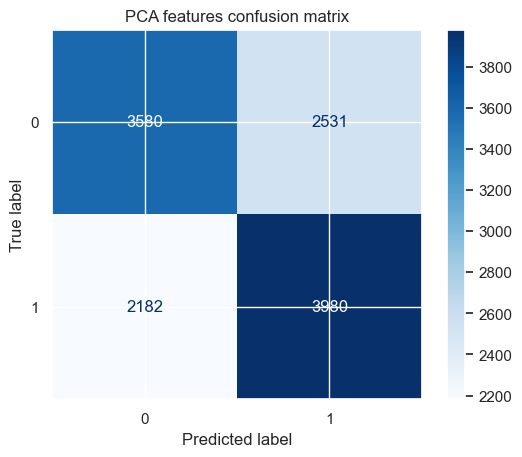
\includegraphics[width=0.6\textwidth]{pca_features_confusion_matrix}
	\caption{Matriz de confusión resultante tras la evaluación de KNN con atributos seleccionados por PCA.}
	\label{Fig: PCACM}
\end{figure}

\begin{table}[htbp]
	\centering
	\caption{Métricas de desempeño del algoritmo KNN con atributos seleccionados por PCA.}
	\begin{tabular}{cccc}
		\hline\hline
		Exactitud    & Sensibilidad   & Precisión & Puntaje F1    \\ 
		\hline\hline
		61.60\% & 64.59\% & 61.13\% & 62.81\% \\
		\hline\hline
	\end{tabular}
	\label{Tab: ResPCA}
\end{table}

\newpage
\subsection{KNN con atributos de selección experimental}
Los resultados obtenidos tras la evaluación del algoritmo utilizando los atributos seleccionados mediante la selección experimental pueden observarse en la Figura \ref{Fig: ExpCM} y en la Tabla \ref{Tab: ResExp}

\begin{figure}[htbp]
	\centering
	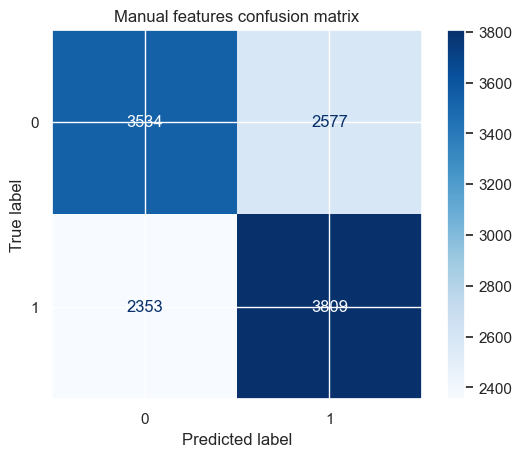
\includegraphics[width=0.6\textwidth]{manual_features_confusion_matrix}
	\caption{Matriz de confusión resultante tras la evaluación de KNN con atributos seleccionados mediante selección experimental.}
	\label{Fig: ExpCM}
\end{figure}

\begin{table}[htbp]
	\centering
	\caption{Métricas de desempeño del algoritmo KNN con atributos seleccionados de forma experimental.}
	\begin{tabular}{cccc}
		\hline\hline
		Exactitud    & Sensibilidad   & Precisión & Puntaje F1    \\ 
		\hline\hline
		59.83\% & 61.81\% & 59.65\% & 60.71\% \\
		\hline\hline
	\end{tabular}
	\label{Tab: ResExp}
\end{table}
